%!TEX root = ../thesis.tex
%*******************************************************************************
%****************************** Second Chapter *********************************
%*******************************************************************************

\chapter{General physical properties 2D materials \label{chap:3}}

\ifpdf
    \graphicspath{{Chapter3/Figs/Raster/}{Chapter3/Figs/PDF/}{Chapter3/Figs/}{Chapter3/Figs/Vector/}}
\else
    \graphicspath{{Chapter3/Figs/Vector/}{Chapter3/Figs/}}
\fi

\section{Structural properties}
\subsection{Layer structure}
\subsection{sp hybirdization}
\subsubsection{Coulson’s theorem}
\subsection{Isotropic v.s. Anisotropic monolayer}
\subsection{Multiphase allotropes}

\section{Electronic properties}
\subsection{Polar bond}
\subsection{Importance of crystal symmetry}

To understand this symmetry, we first need to discuss the hybridization of bonds. C atom has six electron, where two of them strongly localized near the nuclei core, they are called core electrons, such that their interaction with other electrons from other C atoms are suppressed. This only left us with four valence electrons to interact with others and then form bonds. As shown in \autoref{fig:gra_sp2}, the $s$ orbital will hybrid with $p_x$ and $p_y$ orbitals and form three equivalent $sp2$ hybridized orbitals. They repel each other to have a maximum distance between one and the other. Therefore, an optimal angle between them is 120\textdegree, it will lead to the honeycomb structure of graphene. The $p_z$ orbital left unchanged. 

\begin{figure}[htbp!] 
\centering  
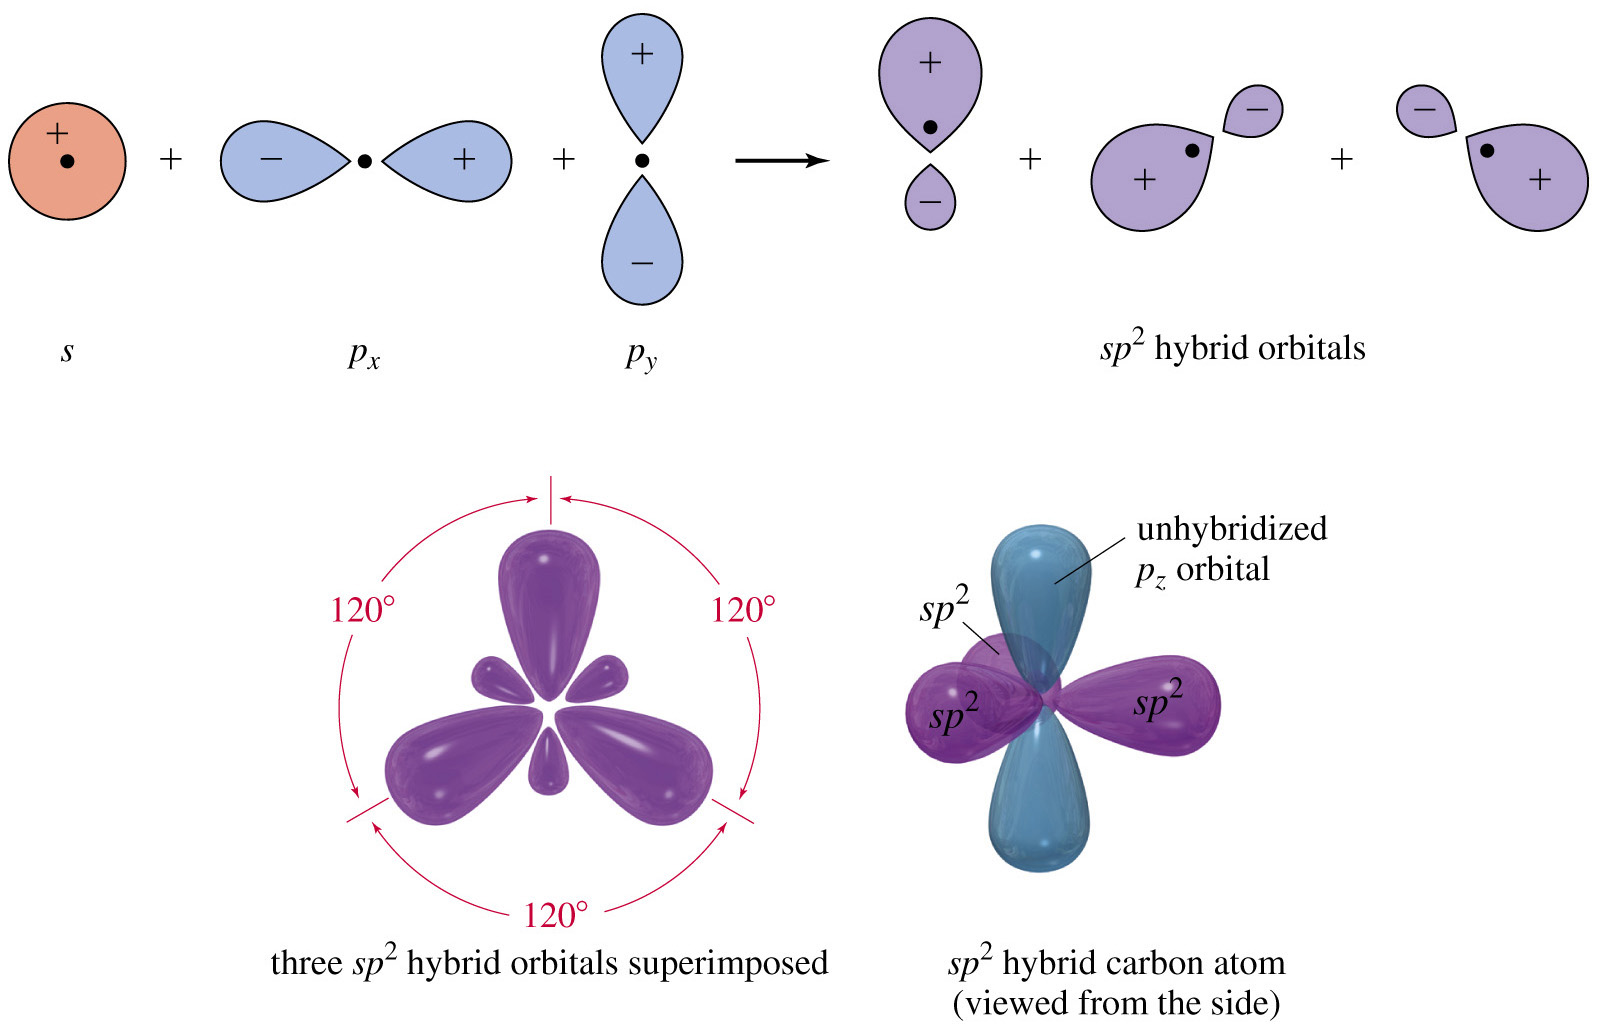
\includegraphics[width=\textwidth]{sphybird}
\caption{The formation of $sp^2$ hybridized orbitals with unhydridized $p_z$ orbital. Image source: \cite{gra_sp2}. }  
\label{fig:gra_sp2}
\end{figure} 

Now C atoms are ready for bonding. The results of bonding is shown in \autoref{fig:gra_bond}. One $sp2$ hybridized orbital with another one from adjacent atom form strong $\sigma$ bond, while $p_z$ orbitals form $\pi$ bonds. It may look like an alternative single and double bonds between atoms, actually the bond order in graphene is 4/3 and it is uniform. We will talk about how a delocalized $\pi$ bond is more stable than alternative single and double bonds in the later chapter where Clar's theory is discussed.

\begin{figure}[htbp!] 
\centering  
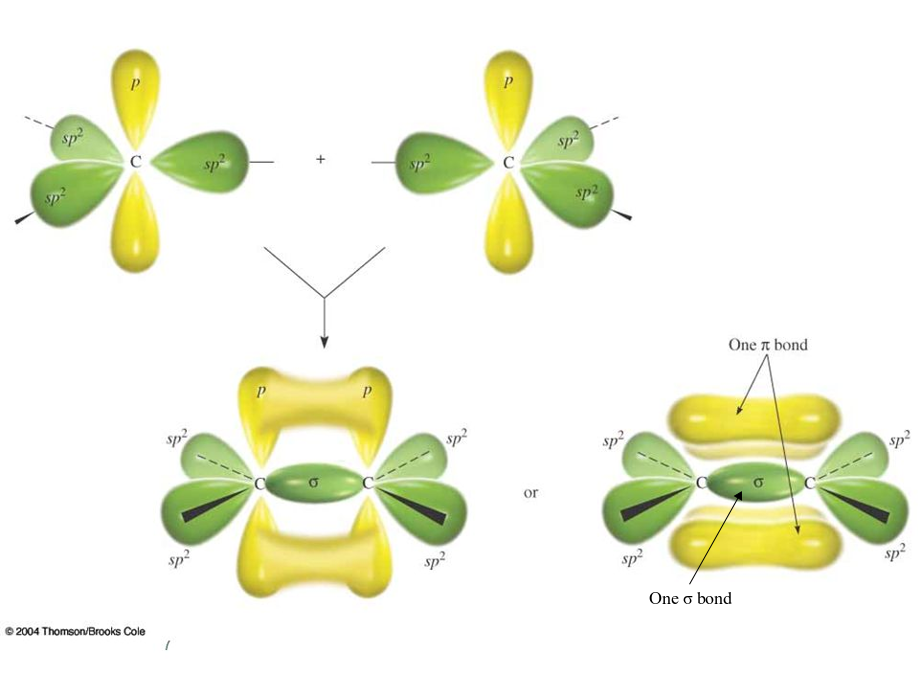
\includegraphics[width=\textwidth]{double_bond}
\caption{The formation of $sp^2$ $\sigma$ and $p_z$ $\pi$ double bond. Image source: \cite{gra_bond}. }  
\label{fig:gra_bond}
\end{figure} 



\begin{figure}[htbp!] 
\centering  
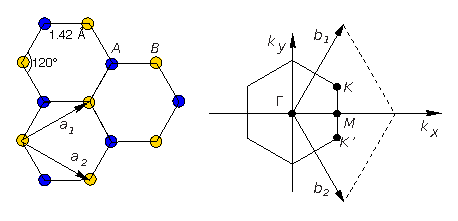
\includegraphics[width=\textwidth]{gra_lat.eps}
\caption{Graphene lattice and its Brillion zone. Image source: \cite{CastroNeto2009}. }  
\label{fig:gra_lat}
\end{figure} 

Every atom has same local environment, however, adjacent atoms are not equivalent. They belong to different hexagonal sublattices $A$ and $B$ as indicated with blue and yellow colors in \autoref{fig:gra_lat}. $a_1$ and $a_2$ are the basis vectors in real space connecting equivalent sites. $b_1$ and $b_2$ are the basis vectors in reciprocal space connecting equivalent k-points. The hexagon in the reciprocal space is the first Brillouin zone where all inequivalent k-points are contained. These kpoints associate with different parallel lines of atoms and thus also indicate different directions in the real space. The k wave vectors near the $\Gamma$ point have longer wave length, while those at the boundary of the first Brillouin zone have wave length that is two times the unitcell dimension on that direction. For example, the most interesting k-point for graphene is the $K$ and $K'$ points. These directions correspond to the $a_1$ and $a_2$ directions in real space. It is only at these k-points in the Brioulloin zone, the antibinding and bonding $\pi$ band touch each other. 



As compared to $\pi$ bond, $\sigma$ bond originate from strong overlap of $sp^2$ orbitals. The interaction is strong and the splitting of bonding and antibonding orbitals are large. Which makes the $\sigma$ bonding orbitals deep in energy, or in other word, makes it strong and difficult to break. This feature contribute the most to the mechanical strength of graphene. On the other hand, $p_z$ orbitals are less overlapped. This makes the $pi$ bond energy close to Fermi level, i.e. the highest occupied state. Therefore, they contribute the most to the electronic properties of graphene.  

\subsubsection{Clar’s theory}
\subsection{Importance of interlayer interaction}
\subsection{Accurate description from DFT}

\section{Vibrational properties}
\subsection{Phonon dispersion of 2D materials}
\subsection{Dynamic stability from phonon dispersion}

\section{Mechanical properties}
\subsection{Elastic and engineering constants}
\subsection{Mechanical stability: Born stability criteria}